%% Speech Communication submission using Elsevier CAS v2.4 (cas-dc).
\documentclass[a4paper,fleqn]{cas-dc}
\usepackage[authoryear]{natbib}
\setlength{\emergencystretch}{2em}

\graphicspath{{../figures/}}

\begin{document}
\let\WriteBookmarks\relax
\def\floatpagepagefraction{1}
\def\textpagefraction{.001}

\shorttitle{Source-validation invariance in cross-corpus SER}
\shortauthors{P. Singh and P. Singh}

\title[mode=title]{What source validation cannot see:
  an affine adaptation audit for cross-corpus speech emotion recognition}

\author[1]{Prashant Singh}[orcid=0009-0001-8585-6005]
\cormark[1]
\fnmark[1]
\ead{2023mcb1309@iitrpr.ac.in}

\author[1]{Pranav Singh}[orcid=0009-0007-3589-6344]
\fnmark[1]

\affiliation[1]{organization={Indian Institute of Technology Ropar},
  city={Rupnagar},
  state={Punjab},
  postcode={140001},
  country={India}}

\cortext[1]{Corresponding author}
\fntext[1]{These authors contributed equally to this work.}

\begin{abstract}
Source-side validation avoids target-label leakage in cross-corpus speech
emotion recognition, but can be invariant to an adaptation operation that
changes target predictions. We establish this property for source translations
and stationary-kernel classifiers: translating source training and validation
together preserves their kernel matrices while shifting the target decision
function. A retrospective audit of frozen RAVDESS and CREMA-D runs finds exact
equality of the selected validation score and hyperparameters in all 30 matched
RBF-SVM cells per direction. Mean matching improves target macro-F1 in every
matched cell, with mean gains of $0.1342$ and $0.1969$ against chance baselines
of $0.1665$ and $0.1656$. Logistic regression, a linear SVM and an MLP are
reported as implementation contrasts outside the proposition's assumptions and
do not generally retain exact numerical equality. We then factor affine
adaptation into relative domain transport and common classifier coordinates.
The factorisation shows why domain-wise standardisation also changes effective
regularisation and kernel geometry, so the broader alignment comparison cannot
isolate the benefit of matching additional moments. The contribution is an
executable audit of what a selection criterion and an affine comparison can
identify, not a new recogniser or an unsupervised target-risk estimator.
The empirical evidence is limited to two English acted-speech corpora; the
analytic claims require the stated kernel and fitting assumptions.
\end{abstract}

\begin{keywords}
speech emotion recognition \sep cross-corpus \sep domain adaptation \sep
distribution alignment \sep self-supervised speech representations \sep
model selection
\end{keywords}

\maketitle

\section{Introduction}
\label{sec:introduction}

Deploying a speech emotion recogniser on a new corpus requires choosing a
model, and often an adaptation operation, without labelled examples from the
deployment corpus. The standard safe answer is to select on held-out
\emph{source} data. That answer is procedurally correct: it touches no target
label, and it cannot leak. This paper asks whether it is also informative, and
shows that for one precisely characterised family of adaptation operations it
is not, in the strongest possible sense.

Consider translating every source training and validation vector by a fixed
offset while leaving target vectors alone. For a classifier whose fit depends
on the source features only through a stationary kernel matrix, that
translation leaves every source-validation prediction unchanged, because the
kernel depends only on differences. The target decision function becomes
$f_0(x-\delta)$, so target predictions can change. The criterion is therefore
exactly constant along a family of different target decision functions. This is
not sampling noise: a larger labelled source-validation set cannot break a
symmetry that holds identically for every sample.

The frozen RAVDESS and CREMA-D grid in this study contains a direct test. In
each direction, all 30 matched RBF-SVM cells have exactly equal stored
validation scores \emph{and} exactly equal selected hyperparameters for
\texttt{none} and \texttt{mean\_shift}, while mean shift changes target
macro-F1 in every one of them. The audit is retrospective and reads only
already-recorded scores; it is reported as such throughout.

The result must not be read as a claim about affine adaptation in general, and
two things stop it. First, its assumptions are specific: logistic regression, a
linear SVM and an MLP appear in the same audit and do \emph{not} retain exact
equality, exactly as a penalised intercept and iterative optimisation predict.
Second, domain-wise standardisation and CORAL do not merely translate. We
factor an affine adaptation into relative domain transport and a common change
of coordinates, and show that the common part also changes the classifier's
effective regularisation and the geometry in which any discrepancy is measured.
A ladder of methods ordered by ``moments matched'' is therefore not a ladder of
otherwise-identical pipelines, and a reported reduction in discrepancy is
defined only relative to a stated basis and bandwidth.

\paragraph{What is and is not new.} Cross-corpus degradation in speech emotion
recognition, the insufficiency of marginal invariance for successful
adaptation, and the difficulty of unsupervised model selection under domain
shift are all established
\cite{schuller2010cross,zhao2019invariant,you2019selection,ericsson2023practices,hu2024selection}.
We claim none of them. The affine reparameterisation is elementary and is
already implicit in the CORAL account \cite{sun2016coral}. What is new is the
identification of an \emph{exact} symmetry of a leakage-free selection
criterion under stated assumptions, its confirmation in a controlled speech
emotion recognition ledger, and the coordinate argument that bounds how far
either result travels.

\paragraph{Contributions.}
\begin{enumerate}
 \item A source-translation invariance for stationary-kernel validation, with
   its fitting assumptions, its consequence for selection, and the numerical
   boundary at which it stops holding
   (Section~\ref{sec:translation-theory}).
 \item An executable, read-only audit of matched frozen runs that tests the
   predicted equality without rounding and without target-based cell
   selection, covering every classifier family with balanced cells so that the
   boundary is measured rather than asserted
   (Sections~\ref{sec:results-translation} and~\ref{sec:results-boundary}).
 \item A factorisation separating relative transport, classifier coordinates
   and measurement geometry, which states what a broader affine comparison and
   its discrepancy diagnostics can and cannot identify
   (Sections~\ref{sec:affine-factorisation} and~\ref{sec:results-frames}).
\end{enumerate}

The paper proposes no recogniser and claims no state-of-the-art performance. It
does not supply an unsupervised estimator of target risk; it characterises a
blind spot in a criterion that is widely used precisely because it is safe. The
analytic statements carry explicit assumptions, the empirical evidence is two
English acted-speech corpora, and the central audit was designed after the
ledger it reads was frozen.

\section{Related work}
\label{sec:related}

\subsection{Cross-corpus speech emotion recognition}
\label{sec:related-crosscorpus}

Cross-corpus SER and strategies for handling corpus variation are established
research problems \cite{schuller2010cross}. Approaches include transfer
learning \cite{naderi2023cross}, multi-task learning \cite{fu2023cross},
training-strategy changes \cite{pastor2023cross}, adversarial adaptation
\cite{latif2023self}, and feature alignment \cite{naeeni2025feature}.
A recent \emph{Speech Communication} study combines class-sensitive feature
dictionaries with an adversarial discriminator in a semi-supervised network
\cite{zhang2025sdan}. It learns representations with additional target
supervision, unlike the frozen source-only affine maps examined here.

Frequently used corpora include IEMOCAP \cite{busso2008iemocap}, RAVDESS
\cite{livingstone2018ryerson} and CREMA-D \cite{cao2014crema}. Their label
mappings, speakers, elicitation procedures and evaluation protocols differ.
Reported scores therefore cannot be ranked without controlling those choices.
EmoBox \cite{ma2024emobox} addresses reproducible cross-corpus evaluation.
Another benchmark alone would not distinguish the present paper. Our question
concerns information available to the model-selection criterion.

\subsection{Alignment and the limits of marginal matching}
\label{sec:related-alignment}

Under covariate shift, the feature marginal changes while the conditional
label distribution is stable \cite{shimodaira2000covariate}. Domain adaptation
also studies settings outside this assumption. A standard target-error bound
contains source error, a domain divergence and the error of the best joint
hypothesis \cite{bendavid2010theory}. Its divergence is classifier-induced,
defined over the symmetric difference of the hypothesis class. Reducing a
kernel two-sample statistic alone need not reduce that divergence or the
joint-error term.

CORAL matches covariance structure \cite{sun2016coral}, and Deep CORAL makes
this a representation-learning objective \cite{sun2016deep}. MMD compares
kernel mean embeddings \cite{gretton2012kernel}; deep adaptation networks
apply multi-kernel matching to learned features \cite{long2015dan}.
Domain-adversarial networks instead use a domain classifier
\cite{ganin2016dann}. These are different adaptation objectives, not a nested
sequence of interventions on moments alone.

Marginal invariance with low source error is already known to be insufficient
for successful adaptation \cite{zhao2019invariant}. We do not claim discovery
of that failure. Our exact result concerns a validation symmetry within a
specified family of source transformations. The affine factorisation
clarifies why it does not automatically apply to the other conditions.

\subsection{Speech representations and layer choice}
\label{sec:related-ssl}

HuBERT, wav2vec 2.0 and WavLM supply the frozen features in this study
\cite{hsu2021hubert,baevski2020wav2vec,chen2022wavlm}. Final-layer pooling and
learned layer aggregation are established choices \cite{yang2021superb}.
Layer-wise probing also shows that the information represented by a speech
encoder changes with depth \cite{pasad2021layer}. The retained layer
comparisons provide context for the criterion audit. They are not presented
as the discovery that intermediate speech representations can be useful.

\subsection{Unsupervised model selection}
\label{sec:related-protocol}

Selecting hyperparameters on target test scores gives an optimistic,
non-deployable estimate. Selection bias is a general evaluation issue
\cite{cawley2010selection}. Deep Embedded Validation
\cite{you2019selection}, the study of validation practice by
\cite{ericsson2023practices}, and the reliability study of
\cite{hu2024selection} already address model selection in domain adaptation.
Their criteria use or evaluate signals beyond the source-validation score
of a single candidate. Our restricted invariance result does not invalidate
these criteria or imply that no unsupervised selector can work.

\subsection{Position of this work}
\label{sec:related-position}

The nearest methodological precedents concern adaptation model selection, not
only SER benchmarking. We contribute a concrete criterion audit: an exact
source-translation invariance, a matched-run check, and a coordinate account
that limits its extension to other affine operations. The reparameterisation
identities are elementary and the underlying selection problem is established.
Their role is to make this SER result interpretable and independently
checkable, not to claim a new general theory of adaptation.

\section{What source validation can identify}
\label{sec:selection-theory}

An adaptation rule can change the target decision function without changing
any source-validation prediction. This section gives an exact example and
then separates it from transformations for which the invariance does not hold.
Features are row vectors. All maps are fitted on source training and
unlabelled target adaptation data, never on target test data.

\subsection{A source-translation invariance}
\label{sec:translation-theory}

Consider a candidate offset $\delta$. Add it to every source-training and
source-validation vector, but leave target vectors unchanged. Mean matching
chooses $\delta=\mu_t-\mu_s$; the argument holds for any fixed offset.

\paragraph{Proposition 1: stationary-kernel validation.}
Let a kernel classifier use $k(x,y)=\psi(x-y)$. Suppose fitting and tie-breaking
depend on the source features only through the training Gram matrix, with
identical labels, hyperparameters and random state. Translating all source
vectors by $\delta$ leaves every source-validation score unchanged. Its target
decision function satisfies
\begin{equation}
 f_\delta(x)=f_0(x-\delta).
 \label{eq:translation-kernel}
\end{equation}
This statement holds for each candidate in a fixed hyperparameter search, not
only for the selected candidate.

\paragraph{Proof.}
Training entries obey $k(x_i+\delta,x_j+\delta)=k(x_i,x_j)$. Validation entries
obey the same identity because both arguments are translated. The fitted
coefficients, intercept and validation predictions are therefore unchanged
under the stated fitting rule. For an unshifted target vector,
$k(x_i+\delta,x)=k(x_i,x-\delta)$. Substitution into the fitted kernel expansion
gives Equation~\ref{eq:translation-kernel}. The argument applies separately
to each binary decision function in a multiclass SVM.

\paragraph{Consequence for selection.}
Even an arbitrarily large labelled source-validation set cannot distinguish
these offsets using the classifier's predictions on that set. A deterministic
tie-break can choose an offset, but its validation score supplies no evidence
that this offset has the best target risk. Target predictions can change when
$x-\delta$ crosses a decision boundary. This is a limitation of this criterion,
not an impossibility result for selectors that also use unlabelled target
features, additional assumptions, or target supervision.

\paragraph{Linear objectives and numerical limits.}
The same phenomenon occurs for an affine head $xW+q$ trained with a loss on
source predictions and a penalty on $W$ alone. Replacing $q$ by $q-\delta W$
preserves every translated-source score and the penalty. Corresponding optima
therefore have the same source risk but can have different target scores.
This is an objective identity, not a guarantee about finite optimisation.
Penalising the intercept breaks it. The implemented \texttt{LinearSVC} uses a
penalised synthetic intercept; neural initialisation, weight decay and early
stopping also prevent an unrestricted invariance claim. Logistic regression
with an unpenalised intercept satisfies the ideal objective assumptions, but
its finite solver can return different numerical solutions. We report that
contrast rather than treating it as an exception to be discarded.

\subsection{Separating transport from classifier coordinates}
\label{sec:affine-factorisation}

The translation result does not imply that validation is invariant to
standardisation or CORAL. To state the distinction, write the two domain maps
as $T_s(x)=xA+a$ and $T_t(x)=xB+b$, where $B$ is invertible. Define
\begin{equation}
 R=AB^{-1},\qquad r=(a-b)B^{-1}.
 \label{eq:relative-transport}
\end{equation}
Then $T_s(x)=(xR+r)B+b$. Thus $xR+r$ is the source transport expressed in
original target coordinates, followed by a common coordinate map $zB+b$.
The source matrix $A$ need not be invertible. This covers source-only affine
maps, whose target map is the identity.

\paragraph{Lemma 2: the induced geometries.}
For a head $zW+q$, let $V=BW$, $u=bW+q$, and $G=BB^\top$. Source scores become
$(xR+r)V+u$ and target scores become $xV+u$. A Euclidean coefficient penalty
and an RBF distance in the transformed coordinates become
\begin{align}
 \lVert W\rVert_F^2 &= \operatorname{tr}(V^\top G^{-1}V),
 \label{eq:penalty-pullback}\\*
 \lVert(x-y)B\rVert^2 &= (x-y)G(x-y)^\top.
 \label{eq:kernel-pullback}
\end{align}
The identities follow by substituting $W=B^{-1}V$ and expanding the squared
norm. The common map therefore induces inverse metrics for the coefficient
penalty and the feature distance. They are not additional alignment methods.

These elementary reparameterisations are not presented as new linear algebra.
Feature/weight equivalence is already part of the CORAL account
\cite{sun2016coral}. Their use here is to specify what the experimental
comparison holds fixed. Equal trial counts and equal scalar regularisation
ranges do not generally equalise an anisotropic penalty matrix. Nor does a
scalar RBF bandwidth search remove arbitrary anisotropy. Equivalence of
objectives also does not imply identical optimisation trajectories.

\paragraph{Why z-score is not a moment-only control.}
Let $D_s,D_t$ contain the effective positive standard deviations used by the
implementation, including its constant-dimension replacements. Domain-wise
z-score has
\begin{equation}
 \begin{split}
 R&=D_s^{-1}D_t,\qquad r=\mu_t-\mu_sR,\\
 B&=D_t^{-1},\qquad b=-\mu_tD_t^{-1}.
 \end{split}
 \label{eq:zscore-factorisation}
\end{equation}
It is diagonal moment transport followed by common target standardisation.
In raw target coordinates its weight penalty uses $D_t^2$, while its distance
metric uses $D_t^{-2}$. A classifier with an isotropic penalty fitted directly
on diagonal moment-matched features is generally a different learner.
Consequently, the existing alignment comparison measures complete pipelines.
It does not isolate the causal contribution of matching additional moments.

\subsection{What a discrepancy comparison measures}
\label{sec:audit-measurement}

Equation~\ref{eq:kernel-pullback} also applies to an MMD kernel. For a change
of common coordinates, keeping Euclidean distance in the new coordinates
changes the kernel in the old coordinates. Conversely, if the intention is
only to express a fixed metric $H$ in coordinates $z'=zQ$, its representation
must change to $Q^{-1}HQ^{-\top}$. These are different measurement questions.
Forcing invariance to every invertible map is not a universal solution;
representation-comparison research shows that excessive invariance can discard
useful information \cite{kornblith2019similarity}.

We therefore audit three objects separately: relative transport $(R,r)$,
the classifier objective in those coordinates, and the diagnostic kernel.
The existing corpus scores cannot retrospectively separate their causal
effects. They can test the exact translation prediction, demonstrate the
failure of a particular source-validation criterion, and quantify sensitivity
to specified measurement protocols. No new alignment algorithm is required
for those questions.

\section{Method}
\label{sec:method}

This section specifies the experimental design in enough detail to reconstruct
it. Where a choice was contestable we state the alternative and why it was
rejected, because several of the conclusions below depend on choices that a
reader may reasonably want to overturn.

\subsection{Corpora and label space}
\label{sec:corpora}

We use two English corpora: RAVDESS \cite{livingstone2018ryerson}
(24 speakers, 1440 utterances, 1.48\,h, mean duration 3.70\,s) and CREMA-D
\cite{cao2014crema} (91 speakers, 7442 utterances, 5.26\,h, mean duration
2.54\,s). Both are publicly available, both carry speaker identity for
every utterance, and their categorical label sets share a six-class
intersection large enough to evaluate per-class transfer. The pairing also
admits a source-size control: capping the larger training split to the smaller
lets each direction be run
at matched training-set size (Section~\ref{sec:splits}), so a reported
asymmetry between directions is not attributable to source-training-set size
alone. Both directions are evaluated.

Both are elicited from actors rather than recorded spontaneously.
Section~\ref{sec:limitations} takes up what that does and does not license.

The shared label space is the six-class intersection
$\{$angry, disgust, fear, happy, neutral, sad$\}$, in alphabetical order, which
is also the index order of every confusion matrix we report. Two mapping
decisions affect the priors and are stated because they are contestable.

\emph{RAVDESS \texttt{calm} is merged into \texttt{neutral}}, since calm exists
only in RAVDESS and cannot transfer. Merging gives neutral 288 utterances
against 192 for every other class; dropping would leave it at 96. Neither
option is balanced. The original speech subset is also not balanced across
all eight labels: neutral has 96 utterances, while each other label has 192.
\emph{RAVDESS \texttt{surprised} is excluded} as it has no CREMA-D counterpart,
removing 192 utterances and leaving 1248. CREMA-D contributes all 7442.
Table~\ref{tab:corpora} gives the resulting statistics.

\begin{table*}[!t]
  \centering
  \caption{Corpora and the mapped six-class intersection. Speakers, utterances and durations describe the raw speech subsets; the last six columns are mapped class priors. Merging RAVDESS \texttt{calm} changes the neutral prior.}
  \label{tab:corpora}
  \begin{tabular}{lrrrrrrrrrrr}
    \toprule
    corpus & spk & utts & hours & mean dur (s) & $n$ (6-class) & \texttt{angr} & \texttt{disg} & \texttt{fear} & \texttt{happ} & \texttt{neut} & \texttt{sad} \\
    \midrule
    RAVDESS & 24 & 1440 & 1.48 & 3.70 & 1248 & 0.154 & 0.154 & 0.154 & 0.154 & 0.231 & 0.154 \\
    CREMA-D & 91 & 7442 & 5.26 & 2.54 & 7442 & 0.171 & 0.171 & 0.171 & 0.171 & 0.146 & 0.171 \\
    \bottomrule
  \end{tabular}
  \\[2pt]
  \begin{minipage}{\linewidth}\footnotesize Derived from \texttt{data/manifest.csv}. RAVDESS \texttt{surprised} (192 utterances) is excluded as having no CREMA-D counterpart; RAVDESS \texttt{calm} is merged into \texttt{neutral}. Neither the original eight-label subset nor this six-class intersection is exactly balanced.\end{minipage}
\end{table*}


Class priors are close but not identical: RAVDESS carries $0.231$ neutral and
$0.154$ for each remaining class, against CREMA-D's $0.146$ and $0.171$.
The neutral mapping changes these empirical priors. It does not establish
that all corpus differences arise from the mapping. Section~\ref{sec:decomposition}
reports prior divergence and the separate label-harmonisation controls.

\paragraph{Label-harmonisation robustness protocol.} We pre-specified two
focused controls. The first sets \path{ravdess_calm_to_neutral=false},
drops the 192 RAVDESS \texttt{calm} utterances, and retains the six-class
intersection. The second also excludes \texttt{neutral} from both corpora,
forming the five-class space \texttt{five\_no\_neutral}. Each mapping has its
own label-map hash, split specification, result ledger and run identifiers. The
controls use cached HuBERT final-layer vectors, logistic regression, five
speaker-disjoint seeds, and the \texttt{none}, \texttt{zscore},
\texttt{mean\_shift} and \texttt{coral} rungs ($\varepsilon=10.0$). Source
validation selects each classifier exactly as in the main protocol. These are
label-harmonisation robustness controls, not replacements for the full
classifier grid.

\subsection{Splits and leakage control}
\label{sec:splits}

Each corpus pair is partitioned into four roles. The source corpus yields
\texttt{source\_train} and \texttt{source\_val}; the target corpus yields
\texttt{target\_adapt} and \texttt{target\_test}. Partitioning is
\textbf{speaker-disjoint} throughout: no speaker appears in more than one role.

The separation between \texttt{target\_adapt} and \texttt{target\_test} is the
central design constraint. Alignment methods require target-domain features by
construction, and they are given \texttt{target\_adapt} only.
\texttt{target\_test} is read exactly once per run, at scoring time, and never
by any fitted object. This is enforced rather than described: every alignment
object records the utterance identifiers it was fitted on, and an assertion
runs on the \emph{real fitted object in every run}, not on a mock and not once
at start-up. Model selection likewise never sees target data; the selection
routine is not passed target features at all, and the target score is computed
afterwards, by the caller, from a model already chosen. Four leakage assertions
hold over all 20 splits (4 pairs $\times$ 5 seeds): no group appears in more
than one split within a corpus; no utterance appears in both a source and a
target split; \texttt{target\_test} never appears in any fitted alignment
object; and the label mapping is a pure function.

At seed 0, RAVDESS $\rightarrow$ CREMA-D gives 988 / 260 / 3765 / 3677
utterances across the four roles, and CREMA-D $\rightarrow$ RAVDESS gives
5972 / 1470 / 624 / 624. Sizes vary slightly across seeds within the
speaker-disjoint constraint.

\paragraph{Matched-$n$ reverse direction.} The two directions differ sixfold in
training-set size, so any asymmetry between them would be confounded with the
amount of source data. We therefore cap \texttt{source\_train} to the smaller
direction's size per seed, subsampling CREMA-D from 5972 to 988: stratified by
class with largest-remainder allocation, so the prior is preserved to within
one utterance per class, and drawn from within the existing speaker-disjoint
split, so utterances are only removed and never moved between roles. Every
leakage guarantee therefore still holds, and the cap is derived per (pair, seed)
rather than hard-coded. \textbf{Both directions reported here are matched in
source-training size only}; a full-$n$ reverse arm was not run.
Source-validation, target-adaptation and target-test sizes remain different
between directions. Consequently this control removes one important
data-quantity confound but does not license an attribution of every directional
asymmetry to corpus properties.

\subsection{Features}
\label{sec:features}

Audio is resampled to 16\,kHz mono and peak-normalised. Three self-supervised
base models are used as frozen feature extractors: HuBERT Base
\cite{hsu2021hubert}, wav2vec 2.0 Base \cite{baevski2020wav2vec} and WavLM Base
\cite{chen2022wavlm}, each providing a CNN encoder output plus twelve
transformer layers, i.e.\ 13 hidden states of dimension 768.

\textbf{All 13 layers are cached}, not only the final one. Final-layer pooling
is the common default and is what the earlier version of this work used;
caching every layer makes depth a searchable condition instead.
Section~\ref{sec:results-aggregation} shows that this choice is worth more than
any choice \emph{among} alignment methods, though less than the decision to
align at all; so it is the axis practitioners may leave at its default while
tuning an axis whose observed differences are smaller in this study.

Two poolings are stored. \emph{Mean pooling} over time gives one 768-d vector
per utterance per layer, used by the four non-sequential classifiers.
\emph{Segment pooling} into 8 uniform temporal segments gives an
$8 \times 768$ sequence, so the Transformer head receives genuine sequence
structure; this costs $8\times$ storage and is the reason that arm exists at
all. Extraction runs at batch size 1 so no utterance is padded against a longer
neighbour: padding would place silence inside the pooled average, and would do
so unevenly across corpora, since RAVDESS utterances average $1.16$\,s longer
than CREMA-D's. A classical MFCC branch is also cached (13 coefficients with
deltas and delta-deltas, mean- and std-pooled, 78 dimensions) but is unused
here.

\subsection{The alignment ladder}
\label{sec:ladder}

The core comparison contains six feature-space conditions. We retain the term
``rung'' as a condition label, not as a claim that these are nested
moment-matching interventions (Section~\ref{sec:affine-factorisation}). Let
$X_s \in \mathbb{R}^{n_s \times d}$ be source-train features and $X_t$ be
\texttt{target\_adapt} features, with means $\mu_s, \mu_t$ and covariances
$C_s, C_t$. All six rungs are fitted on $X_s$ and $X_t$ only.

\begin{description}
  \item[\texttt{none}] The identity. $x \mapsto x$.
  \item[\texttt{zscore}] Per-dimension standardisation of each domain to zero
    mean and unit variance: $x \mapsto (x - \mu)\oslash\sigma$ within each
    domain. Matches the first and second marginal moments per dimension, with
    no cross-dimension terms.
  \item[\texttt{mean\_shift}] $x \mapsto x + (\mu_t - \mu_s)$. Matches the
    first moment only.
  \item[\texttt{coral}] Whitening by the source covariance and recolouring by
    the target's \cite{sun2016deep}:
    $x \mapsto (x - \mu_s) C_s^{-1/2} C_t^{1/2} + \mu_t$. Matches first and
    second moments including cross-terms in the unregularised idealisation.
    With shrinkage, the identity is $M^\top\tilde C_sM=\tilde C_t$;
    empirical covariances need not match exactly.
  \item[\texttt{mkmmd\_diag}] A learned diagonal affine map minimising a
    multi-kernel MMD objective, defined below.
  \item[\texttt{mkmmd\_full}] The same objective with a full matrix $W$.
\end{description}

\paragraph{Mean matching.} For a linear kernel, the squared distance between
empirical kernel means is $\lVert\mu_s-\mu_t\rVert^2$. Within translations,
its minimising offset is $\mu_t-\mu_s$. Among unrestricted affine maps this
does not uniquely select a translation: any matrix $A$ can match the means
with offset $\mu_t-\mu_sA$. The empirical-mean expression is not the unbiased
finite-sample estimator used for the RBF diagnostics. We name the operation
\texttt{mean\_shift}, not ``MMD''.

\paragraph{Regularisation of CORAL.} With $d = 768$ and roughly one thousand
source-train samples, the rank bound $\min(d,n-1)$ does not itself imply
singularity. Shrinkage stabilises whitening when small eigenvalues make it
ill-conditioned. It is
scale-aware, $\tilde{C} = C + \varepsilon\,\frac{\mathrm{tr}(C)}{d} I$:
anchoring to the mean eigenvalue matters because a fixed absolute ridge means
something different for every backbone and layer. $\varepsilon$ is a
\emph{searched} axis over $\{10^{-4}, \ldots, 10\}$ in decades, selected on
\texttt{source\_val} and recorded on every row, with a Ledoit--Wolf variant
\cite{ledoit2004covariance} as a
parameter-free alternative. Condition number and effective rank are recorded
after regularisation; a matrix still singular there raises rather than being
pseudo-inverted.

\paragraph{Multi-kernel MMD.} The two MK-MMD rungs learn an affine map
$(W, b)$ minimising
\begin{equation}
  \mathcal{L}(W, b) \;=\;
  \mathrm{MMD}^2_k\!\left(X_s W^\top + b,\; X_t\right)
  \;+\; \lambda \lVert W - I \rVert_F^2 ,
  \label{eq:mkmmd}
\end{equation}
where the implementation stores $W$ as the transpose of the row-vector map
used in Section~\ref{sec:affine-factorisation}, and $k$ is a sum of Gaussian
kernels at bandwidth multipliers
$\{0.25, 0.5, 1, 2, 4\}$ of the median pairwise distance
\cite{gretton2012kernel}, and $\mathrm{MMD}^2$ is the unbiased estimator.
\texttt{mkmmd\_diag} constrains $W$ to be diagonal; \texttt{mkmmd\_full} does
not. The identity anchor regularises a full matrix with $\approx 590$k
parameters fitted on about a thousand source samples. It penalises $W-I$,
not $b$. Even an ideal large-$\lambda$ limit therefore leaves a translation
to optimise; it does not necessarily recover \texttt{none}. No asymptotic
optimisation guarantee is claimed for the finite-step procedure.
$\lambda$ is searched over
$\{10^{-3}, \ldots, 10^{2}\}$ in decades.

Optimisation uses Adam \cite{kingma2015adam} for 200 steps at batch size 256,
warm-started from the
CORAL solution (full) or a diagonal moment match (diagonal). The learning rate
is $\eta = \eta_0 / \sqrt{P}$ with $\eta_0 = 0.01$ and $P$ the parameter count:
Adam normalises per parameter, so a fixed rate gives a step whose Frobenius
norm grows as $\sqrt{P}$; for a full $W$, norm $\approx 0.77$ per iteration,
which does not converge.

\paragraph{Fallback, and why it must be reported.} An unpenalised MMD check
on the first 400 observations compares the candidate with its warm start.
If the candidate worsens this check, the returned map reverts to the
warm start. This differs from the penalised minibatch training objective;
rejection is not proof of failure to improve that objective. Optimiser
diagnostics describe the attempted fit, while target scores use the returned
map. Across the main grid the check rejects the candidate
in \textbf{64.9\%} of \texttt{mkmmd\_diag} runs and \textbf{55.2\%} of
\texttt{mkmmd\_full} runs. In those cells the fitted map is the warm start:
the diagonal moment match for \texttt{mkmmd\_diag}, and CORAL for
\texttt{mkmmd\_full}. Reporting either as a distinct learned map without saying
so would overstate what was actually fitted. The rates accompany the ladder
result in Section~\ref{sec:results-ladder} and the generated results document.
They qualify every MK-MMD comparison in this paper: the experiment evaluates
these affine maps, this warm start, and this optimisation budget. It does not
establish what a differently optimised MK-MMD map would achieve.

\subsection{Measuring distribution discrepancy}
\label{sec:discrepancy}

Alignment methods are usually justified by the discrepancy they remove, so the
discrepancy statistic needs to be specified as carefully as the methods.

We report the raw unbiased $\mathrm{MMD}^2$ between aligned source and target
and its effect size, obtained by dividing by the mean absolute $\mathrm{MMD}^2$
over five random source half-splits. The unbiased estimator has null mean zero,
so its signed mean is not a usable denominator. The effect size aids
interpretation of finite-sample variation; it does not replace the raw
statistic.

\paragraph{A common reference geometry.} For the ladder diagnostic, one ZCA
basis is derived from unaligned \texttt{source\_train} features with shrinkage
$\varepsilon = 10^{-2}$. One median RBF bandwidth is then derived from those
same source-train features in that basis. Both quantities are fixed before an
alignment map is fitted and applied identically to every rung for that pair,
seed, backbone and layer aggregation. This makes the raw trajectories a
comparison under one stated kernel and coordinate system. The shrinkage avoids
amplifying near-null directions in the source covariance. A
scale-changing map can nonetheless drive a fixed-bandwidth RBF kernel into
saturation. We report that failure mode rather than treating a near-zero
statistic as evidence of distributional equality.
Each MMD evaluation uses a seeded cap of 128 utterances per sample set; the cap
is identical for the marginal, class-conditional and null computations and is
recorded in every diagnostic row.

\paragraph{Adaptive geometry as a sensitivity analysis.} We separately report
an own-geometry calculation that derives the median bandwidth from each
compared feature pair. The 13-layer frame-sensitivity sweep also holds the ZCA
basis fixed while recomputing that adaptive bandwidth; we call it a
\emph{reference-basis} calculation, not a fully fixed reference geometry. The
two procedures answer different measurement questions, so neither is treated
as the unique definition of distributional closeness.

\paragraph{Proposition: median-heuristic scale invariance.} Let
$\hat\sigma(X,Y)$ be the median pairwise Euclidean distance used by the RBF
kernel. For a nonzero scalar $a$,
$\hat\sigma(aX,aY)=|a|\hat\sigma(X,Y)$ and therefore
\begin{equation}
  k_{|a|\hat\sigma}(ax,ay)=k_{\hat\sigma}(x,y).
  \label{eq:median-scale-invariance}
\end{equation}
Each pairwise distance gains the factor $|a|$, which proves the first identity;
substitution in the RBF exponent proves the second. Thus an adaptive
median-heuristic MMD is invariant to a global rescaling applied to both samples.
This property does not extend to an arbitrary affine map or to a map applied to
only one sample.

\paragraph{Class-conditional diagnostic.} For each class $k$, the analysis
computes the same unbiased multi-kernel MMD$^2$ between aligned
$X_s \mid y=k$ and $X_t \mid y=k$ in the common reference geometry. A class is
undefined rather than estimated when either side has fewer than 50 examples.
The report also gives a class-specific half-split effect size. That normaliser
is not the marginal normaliser, so we do not form or interpret a
conditional-to-marginal ratio. The diagnostic is not a probability
decomposition or an estimate of $P(y \mid x)$.

\subsection{Classifiers and the search budget}
\label{sec:classifiers}

Five families are evaluated: logistic regression, linear SVM, RBF SVM, an MLP,
and a small Transformer head over the 8-segment sequence. Each is searched with
\textbf{exactly the same number of trials}; 20 random-search draws; and
the trial count is recorded on every result row. This controls trial count,
not effective model capacity or coverage of equally favourable settings.

Hyperparameter candidates are drawn by seeded random search. A failed fit
receives score $-\infty$ and is not replaced by an additional draw.

Two further constraints. First, \textbf{no standardisation inside any
classifier}. This preserves the frozen raw-coordinate baseline. A scaler
fitted on source training and shared across domains would be a different
control; it would not equal domain-wise \texttt{zscore}. Consequently this
grid does not isolate alignment from classifier conditioning. Second, the
iteration cap for the iterative solvers is a fixed convergence budget
($2\times10^4$) rather than a searched hyperparameter, as it was in an earlier
revision: searching it lets a trial win selection by having stopped early
rather than by fitting better. Convergence is asserted rather than warned
about; a fit that reaches the cap is recorded as a failed trial and cannot
be selected; and across the whole grid \textbf{0 of 99{,}720 trials failed
to converge}.

Layer aggregation is a searched condition with three settings: \texttt{last}
(the common default), \texttt{layer:6} (a fixed mid-stack layer), and
\texttt{weighted} (a softmax over all 13 states learned jointly with the head).
The last is implemented only for the two torch families, whose training loops
jointly optimise the layer weights and head. It is not searched for the
scikit-learn classifiers in this implementation.

The Transformer arm is a deliberately \textbf{reduced-seed arm}: two seeds, the
primary direction only, one inner-grid setting per rung. Its per-cell cost is
15--40$\times$ the other families', and carrying it at full width would have
spent more compute on it than on every other axis combined. The full-grid
headline and ladder summaries include its available cells, so the forward
candidate set is not identical across seeds. The matched-direction comparison
in Section~\ref{sec:results-direction} excludes it. The translation audit
uses only the RBF-SVM and logistic-regression families and is unaffected.

\subsection{Selection protocol}
\label{sec:selection}

We report two protocols side by side, and the distinction between them is one
of the paper's results rather than a presentational choice. \textbf{Validated}
is the configuration with the highest \texttt{source\_val} macro-F1 within a
given (pair, seed), scored on \texttt{target\_test}; it is what a practitioner
could actually obtain, using no target labels at any point. \textbf{Oracle} is
the highest \texttt{target\_test} macro-F1 present in the grid for that
(pair, seed): a \textbf{post-hoc target-selected benchmark unavailable to the
deployable source-only selection protocol}. The
validated-to-oracle difference is called the \emph{oracle gap}. It does not
identify a causal effect of source-side selection because it also contains
finite-target-sample noise, search-space size, and optimism from maximising the
target score.

The gap between them is the quantity of interest. Reporting only the oracle
amounts to selecting on target scores. The earlier version of this work did
this. It makes a method look as good as its best run.

\paragraph{How the ladder handles unequal inner grids.} Each result row already
contains the best of its classifier family's 20 source-validation trials. For a
ladder summary, we then hold (pair, seed, backbone, layer aggregation,
classifier family) fixed and select that rung's best remaining inner setting
($\varepsilon$ for CORAL or $\lambda$ for MK-MMD) by
\texttt{source\_val} macro-F1. Target predictions from only these selected
cells enter the paired cluster bootstrap. The row counts in Table~\ref{tab:ladder}
are therefore candidate rows before this second selection, not equally weighted
observations in a rung mean; they differ because the rungs legitimately have
different inner grids.

\subsection{Metrics, baselines and inference}
\label{sec:metrics}

The primary metric is macro-F1 on \texttt{target\_test}. Accuracy and
unweighted average recall are also recorded on every row.

\textbf{Every performance number is reported against its baselines.} An analytic
chance baseline (the expected macro-F1 of a uniformly random classifier, given
the realised target-test priors) and a majority-class baseline are computed on
every row from the realised distribution rather than by simulation. Here the
chance baseline is $0.1665$ (RAVDESS $\rightarrow$ CREMA-D) and $0.1656$
(CREMA-D $\rightarrow$ RAVDESS), and the majority baseline is $0.0425$ and
$0.0444$. A macro-F1 without its baselines is not interpretable, and one number
below its chance baseline is below the expected random-classifier score. Because
the baseline is pair-dependent,
\textbf{no figure in this paper averages macro-F1 across pairs}.
Table~\ref{tab:floors} collects the split sizes and both baselines.

\begin{table}[tb]
  \centering
  \caption{Split sizes and the floors every macro-F1 in this paper is read against. Both directions are matched-$n$: CREMA-D source-train is subsampled from 5972 to match RAVDESS, so a reported asymmetry cannot be a training-set size effect.}
  \label{tab:floors}
  \begin{tabular}{lrrrrrr}
    \toprule
    pair & source\_train & source\_val & target\_adapt & target\_test & chance & majority \\
    \midrule
    RAVDESS $\rightarrow$ CREMA-D & 988 & 260--260 & 3752--3765 & 3677--3690 & 0.1665 & 0.0425 \\
    CREMA-D $\rightarrow$ RAVDESS & 988 & 1470--1476 & 624--624 & 624 & 0.1656 & 0.0444 \\
    \bottomrule
  \end{tabular}
  \\[2pt]
  \begin{minipage}{\linewidth}\footnotesize Ranges span the five seeds within the speaker-disjoint constraint. Floors are analytic from the realised \texttt{target\_test} priors, not simulated. Because the chance floor is pair-dependent, no result in this paper averages macro-F1 across pairs.\end{minipage}
\end{table}


\paragraph{Intervals.} Target-score intervals come from a \textbf{paired
cluster bootstrap} with 2000 replicates \cite{cameron2008cluster}. In each
replicate, we draw the five seed identifiers with replacement. For each drawn
seed, we draw that seed's target-test speaker identifiers with replacement,
keeping every utterance from each selected speaker. Both comparison arms use
the same seed and speaker draws, then their macro-F1 difference is formed. This
resamples the split, search and initialisation variation carried by seeds and
the clustered target-test sampling variation carried by speakers. It never
resamples individual utterances independently.

\paragraph{Why the source-selected summary uses a different interval.} The
paired cluster bootstrap requires a fixed arm: a condition that can be
recomputed on any resampled set of speakers and seeds. The source-selected
summary in Table~\ref{tab:headline} is not such an arm. Its value for a seed is
the target macro-F1 of \emph{whichever} configuration source-side validation
chose on that seed, and the chosen configuration differs across seeds; in the
forward direction the protocol selects \texttt{none} on two of five seeds and an
aligned rung on the other three (Section~\ref{sec:results-selection}). Each seed
therefore contributes one number describing a complete deployment decision, and
those five numbers are summarised by a mean and a 95\% $t$-interval over seeds.

That interval estimates the between-seed variability of the deployable
selection outcome, which includes both the split realisation and the change of
selected configuration it induces. It does \textbf{not} incorporate any further
within-seed resampling of target-test speakers, so it is not comparable to the
paired intervals elsewhere in this paper and is not offered as a better
estimator. It answers a different question: how much the end-to-end protocol
varies from one split to another. Its width is also limited by having five
observations. Fixed-arm contrasts, where both conditions can be recomputed on
identical seed and speaker draws, use the paired cluster bootstrap throughout.
The same estimator is applied to the oracle column and to their difference, so
the three columns of that table are on a common basis.

\paragraph{What the oracle column is.} The oracle is the best target macro-F1
present in the grid for that pair and seed. It is selected using target-test
scores and is therefore not attainable by any source-only protocol; it is a
benchmark for the grid as configured, not a result. Its interval carries the
same maximisation: the maximum of a set of noisy scores is biased upward, so
the oracle column is an optimistic summary of this target set rather than an
estimate of achievable performance. The difference between the two columns is
reported as an \emph{oracle gap} and is descriptive. It is not the causal
effect of using source-side selection, because it also contains target-set
maximisation, finite-sample variation and the extent of the search space.

The discrepancy columns are properties of a fitted map, not of a prediction.
The ladder discrepancy columns are candidate-row means without intervals.
Other discrepancy summaries state their own aggregation. The frame sweep's
cell-and-seed correlations are descriptive because cells share seeds and
feature sets; pooled independence-based intervals are not used as evidence
for a population-level sign change.

\paragraph{AI-assisted code development.} OpenAI Codex was used to assist with
code scaffolding and maintenance. The authors specified the experimental
protocol, reviewed and edited all generated code, ran the tests and experiments,
and verified every reported result against the generated artifacts.

\paragraph{Multiple comparisons.} A primary comparison family of seven
contrasts $\times$ two directions was \textbf{pre-specified in code before the
frozen confirmatory grid was run}: the five ladder rungs against \texttt{none}, and
two layer-aggregation contrasts. Holm-Bonferroni correction
\cite{holm1979sequential} is applied across exactly those 14 tests.
Holm rather than Bonferroni because it is uniformly more powerful at the same
family-wise error rate, and rather than a false-discovery-rate procedure
because the family is small and pre-specified, where controlling the
family-wise rate is the stricter guarantee.

Comparisons outside that family are reported as such, and are never presented
as though they had been pre-specified. Where such a comparison supports a
\emph{null} claim; that some difference is negligible; we report a bound
rather than a test, since failing to reject a null is not evidence for it.
Where one supports a positive claim, correction is applied within that
comparison's own set and both the raw and corrected $p$ are given, so that a
result surviving only before correction is visible as such.

\subsection{Experimental scope}
\label{sec:scope}

The main grid is a reduced factorial; 2 directions $\times$ 3 backbones
$\times$ 5 seeds $\times$ 6 rungs $\times$ layer aggregation $\times$ 5
classifier families, with inner grids over $\varepsilon$ and $\lambda$. This
totals 4986 runs. A smoke gate and a screening stage pruned
only the inner grids on \texttt{source\_val} evidence alone. Three probes
supplement it: a 13-layer sweep (2340 runs), a CORAL shrinkage asymptote probe
(120 runs) and a shift decomposition (120 records). No run failed. Results here
carry the frozen configuration tag \texttt{grid-freeze-v3};
Section~\ref{sec:reproducibility} describes the provenance machinery.

\section{Results}
\label{sec:results}

Numbers come first in each subsection and interpretation is separated from
them. Every macro-F1 is reported against its own pair's chance baseline, and
because that baseline is pair-dependent, nothing is averaged across pairs.
Unless stated otherwise, intervals are 95\% paired cluster bootstrap intervals
over target-test speakers and seeds.

Sections~\ref{sec:results-translation} and~\ref{sec:results-boundary} test
Proposition 1 and delimit it. Sections~\ref{sec:results-selection}
to~\ref{sec:results-aggregation} place that result inside the frozen pipeline
comparison it was found in. Robustness controls and diagnostics whose
interpretation we deliberately restrict are summarised in
Section~\ref{sec:results-robustness} and reported in full in the supplementary
material. Table values and figure data are generated from the retained result
files, and both the original outcome report and the retrospective translation
report are included in the automated manuscript number-trace check.

\subsection{Exact validation equality in the frozen translation pairs}
\label{sec:results-translation}

Table~\ref{tab:translation-audit} tests the stored consequences of
Proposition 1. The audit joins \texttt{none} and \texttt{mean\_shift} by
direction, seed, backbone, layer, classifier, split identifiers and sizes,
and label-map, feature and search hashes. It requires one successful row per
arm and rejects duplicates or unmatched rows. No target score participates
in the join or the inclusion rule. The configuration and input-ledger hashes,
all matched run identifiers and unrounded values are released with the audit.

\begin{table*}[!t]
\centering\small
\caption{Retrospective translation audit on frozen runs. Each cell is one matched \texttt{none}/\texttt{mean\_shift} pair sharing direction, seed, backbone, layer setting, classifier and every split, label-map, feature and search identifier. Equal validation and equal parameters count exact equality of the stored winning source-validation score and the selected classifier parameters. $\Delta$ is mean target macro-F1 for mean shift minus none; Positive counts cells with a target improvement. Chance is the uniform-random baseline. The upper panel is the exact prediction of Proposition 1. The lower panel reports families whose fitting rules fall outside its assumptions, which the proposition does not cover and which are therefore scope evidence rather than counterexamples. Cells share seeds; no independence-based test is reported and no general claim about mean shift follows from the $\Delta$ column.}
\label{tab:translation-audit}
\begin{tabular}{llrrrrrr}
\toprule
Direction & Head & Pairs & Equal val. & Equal params & $\Delta$ & Positive & Chance \\
\midrule
\multicolumn{8}{l}{\textbf{Stationary kernel, Gram-determined fit: Proposition 1 applies}} \\
CREMA-D $\to$ RAVDESS & RBF SVM & 30 & 30 & 30 & +0.1969 & 30 & 0.1656 \\
RAVDESS $\to$ CREMA-D & RBF SVM & 30 & 30 & 30 & +0.1342 & 30 & 0.1665 \\
\midrule
\multicolumn{8}{l}{\textbf{Penalised intercept or iterative solver: outside those assumptions}} \\
CREMA-D $\to$ RAVDESS & Logistic & 30 & 0 & 22 & +0.1881 & 30 & 0.1656 \\
RAVDESS $\to$ CREMA-D & Logistic & 30 & 3 & 12 & +0.1442 & 30 & 0.1665 \\
CREMA-D $\to$ RAVDESS & Linear SVM & 30 & 0 & 19 & +0.1776 & 30 & 0.1656 \\
RAVDESS $\to$ CREMA-D & Linear SVM & 30 & 6 & 15 & +0.1456 & 30 & 0.1665 \\
CREMA-D $\to$ RAVDESS & MLP & 45 & 0 & 24 & +0.1701 & 45 & 0.1656 \\
RAVDESS $\to$ CREMA-D & MLP & 45 & 0 & 12 & +0.1287 & 45 & 0.1665 \\
\bottomrule
\end{tabular}
\\[2pt]
\begin{minipage}{\linewidth}\footnotesize Filter: \texttt{grid-freeze-v3}, \texttt{blending=none}; matched \texttt{none}/\texttt{mean\_shift} rows only. Every family spans three backbones and five seeds; the MLP additionally has the learned \texttt{weighted} layer aggregation, which the closed-form heads cannot use, hence its larger cell count. The reduced-seed transformer arm has no balanced matched cells and is excluded by construction. Generated by \texttt{tools/audit\_translation.py} from the configuration \texttt{configs/audit\_translation.yaml}. The JSON report retains input/configuration hashes and both run IDs for every pair. Means are descriptive, not independent-cell inference.\end{minipage}
\end{table*}


For the RBF SVM, all 30 pairs in each direction have exactly equal stored
winning validation scores and selected hyperparameters. This is the predicted
equality, observed without exception in the arm the proposition covers. Mean
shift improves target macro-F1 in every pair, with directional mean differences
of $+0.1342$ and $+0.1969$. Source-side validation therefore assigned identical
evidence to two conditions whose target predictions differ, which is the
failure the proposition describes.

The ledger stores the winning validation score for each run, not the
predictions of every search candidate. The audit is accordingly a check of the
recorded winning scores and selected parameters, not an empirical verification
of the entire search surface; the statement about every candidate remains
analytic. The analysis is retrospective and uses existing scores only, and
cells share seeds and speakers, so the table reports descriptive paired means
rather than a test treating each cell as an independent replication.

Target macro-F1 favours mean shift in every matched pair of every family. That
is a descriptive property of these frozen cells against an unaligned baseline
in one corpus pair. It is not evidence that mean matching improves cross-corpus
speech emotion recognition in general, and no such claim is made here.

\subsection{What the boundary classifiers show}
\label{sec:results-boundary}

The audit covers every classifier family in the frozen grid with complete,
balanced matched cells. Only the RBF SVM satisfies Proposition 1's fitting
assumptions, and Table~\ref{tab:translation-audit} is drawn in two panels on
that basis. The lower panel reports the three families the assumptions exclude,
identified in advance in Section~\ref{sec:translation-theory}: a penalised
synthetic intercept in the linear SVM, a finite iterative solver in logistic
regression, and initialisation, weight decay and early stopping in the MLP.

They behave as those assumptions predict. Logistic regression has exactly equal
stored validation scores in 3 forward pairs and none in reverse, with selected
hyperparameters agreeing in 12 forward and 22 reverse pairs. The linear SVM has
6 forward and no reverse exact equalities, with 15 and 19 parameter agreements.
The MLP, which additionally searches the learned \texttt{weighted} layer
aggregation and therefore has 45 pairs per direction, has no exact validation
equality in either direction and parameter agreement in 12 forward and 24
reverse pairs.

None of this contradicts Proposition 1, whose statement does not extend to a
penalised intercept or to iterative neural training. These rows are evidence
about the boundary of the proposition, not tests of it. The pattern separates
an exact identity between objectives from the numerical behaviour of the
solvers that approximate them, and it is reported rather than omitted so that
the scope of the proposition rests on the full set of eligible frozen cells.
The reduced-seed transformer arm has no balanced matched cells and is excluded
by construction.

\subsection{What the criterion costs a practitioner}
\label{sec:results-selection}

The invariance in Section~\ref{sec:results-translation} is exact but local: it
concerns two conditions the criterion cannot separate. Table~\ref{tab:headline}
gives the consequence for the whole protocol, comparing the configuration
selected on source-side validation alone against the best configuration present
in the grid. Its intervals are the one exception to the convention stated above:
because the selected configuration differs across seeds, this table reports a
$t$-interval over the five seeds rather than a paired cluster bootstrap.
Section~\ref{sec:metrics} states what that interval does and does not include.

\begin{table}[tb]
  \centering
  \caption{Target macro-F1 of the configuration selected on source validation, against the best configuration present in the grid. The oracle column is an upper bound no protocol can reach and is not a result.}
  \label{tab:headline}
  \begin{tabular}{lrrrrr}
    \toprule
    pair & validated & oracle & gap & chance & majority \\
    \midrule
    RAVDESS $\rightarrow$ CREMA-D & 0.3156 [0.1880, 0.4432] & 0.4555 [0.4326, 0.4785] & 0.1399 [0.0231, 0.2568] & 0.1665 & 0.0425 \\
    CREMA-D $\rightarrow$ RAVDESS & 0.4994 [0.4592, 0.5395] & 0.5680 [0.5148, 0.6212] & 0.0687 [0.0090, 0.1283] & 0.1656 & 0.0444 \\
    \bottomrule
  \end{tabular}
  \\[2pt]
  \begin{minipage}{\linewidth}\footnotesize Filter: \texttt{freeze\_tag=grid-freeze-v3}, \texttt{blending=none}, 4986 runs. Mean over 5 seeds with a 95\% $t$-interval. Both floors are analytic from the realised target-test priors.\end{minipage}
\end{table}


Validated macro-F1 is $0.3156$ $[0.1880, 0.4432]$ for
RAVDESS $\rightarrow$ CREMA-D against a chance baseline of $0.1665$, and
$0.4994$ $[0.4592, 0.5395]$ for CREMA-D $\rightarrow$ RAVDESS against
$0.1656$. The oracle values are $0.4555$ $[0.4326, 0.4785]$ and
$0.5680$ $[0.5148, 0.6212]$; \textbf{the oracle is a post-hoc target-selected
benchmark unavailable to the deployable source-only selection protocol}. The
validated-to-oracle difference is the \emph{oracle gap}: $0.1399$
$[0.0231, 0.2568]$ and $0.0687$ $[0.0090, 0.1283]$. It does not identify a
causal effect of source-side selection, because it also includes target-set
maximisation, finite-sample variation and search-space effects.

Figure~\ref{fig:selection} shows the gap per seed, and the forward direction is
where the protocol visibly fails. Forward, \texttt{source\_val} separates
\texttt{none} ($0.7304$) from \texttt{zscore} ($0.7322$) by $0.0018$, while the
same two rungs differ on target by $0.13$. Unlike the source-translation
result, this near-tie is empirical rather than an exact invariance; the
criterion is not symmetric here, merely uninformative at the resolution
available. The consequence is that selection falls back to \texttt{none} on two
of five forward seeds, returning target macro-F1 of $0.2803$ and $0.1508$.
\textbf{The second is below that pair's chance baseline of $0.1665$.} The
protocol uses no target labels and has no source-side indication of this
outcome. The reverse direction selects an aligned rung on all five seeds
(\texttt{mean\_shift} four times, \texttt{zscore} once) and its gap is
correspondingly smaller.

\begin{figure*}[!t]
  \centering
  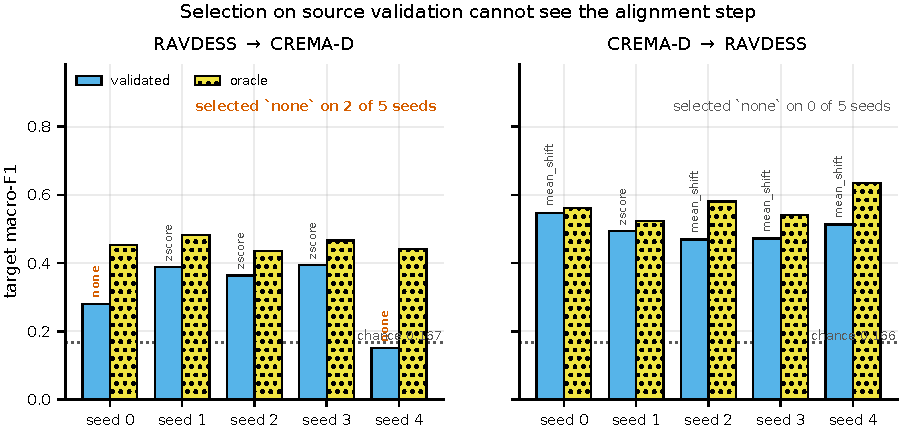
\includegraphics[width=\textwidth]{validated_vs_oracle.pdf}
  \caption{Validated against oracle target macro-F1 for each seed, with the
    rung the protocol selected annotated on each validated bar. In the forward
    direction the protocol selects the unaligned condition on two of five
    seeds; on one of them the result falls below the chance baseline.}
  \label{fig:selection}
\end{figure*}

This result is limited to selecting the alignment condition. It does not
assess source-side selection for layer aggregation, which
Section~\ref{sec:results-aggregation} addresses separately.

\subsection{The affine comparison as pipeline context}
\label{sec:results-ladder}

The conditions the criterion was selecting among are the affine ladder.
Table~\ref{tab:ladder} gives source-selected target macro-F1 by rung alongside
candidate-row discrepancy summaries, and Table~\ref{tab:primary} gives the
pre-specified comparison family. These are different averaging protocols: the
discrepancy columns include every inner setting, whereas target scores use the
source-selected setting in each cell. Their juxtaposition is descriptive and is
not a matched map-level correlation. The forward summaries include available
transformer cells from its reduced-seed arm, so they are not an equal-family,
identical-candidate-set comparison across seeds.

\begin{table*}[!t]
  \centering
  \caption{The alignment ladder. Within each (pair, seed, backbone, layer aggregation, classifier) cell, the source-validation-best inner setting is selected before target scoring. Target macro-F1 rises once, off \texttt{none}, and then does not track discrepancy: \texttt{mkmmd\_full} reaches the lowest discrepancy in both geometries and is never the best rung.}
  \label{tab:ladder}
  \resizebox{\textwidth}{!}{%
  \begin{tabular}{lrrrrr}
    \toprule
    pair & rung & candidate rows & target macro-F1 & effect (own) & effect (ref) \\
    \midrule
    RAVDESS $\rightarrow$ CREMA-D & \texttt{none} & 153 & 0.2289 [0.2133, 0.2444] & 1432.93 & 36905.40 \\
     & \texttt{zscore} & 153 & 0.3599 [0.3483, 0.3726] & 51.79 & 480.85 \\
     & \texttt{mean\_shift} & 153 & 0.3595 [0.3442, 0.3762] & 104.05 & 19641.52 \\
     & \texttt{coral} & 828 & 0.3648 [0.3480, 0.3831] & 34.84 & 311.15 \\
     & \texttt{mkmmd\_diag} & 558 & 0.3497 [0.3347, 0.3663] & 67.34 & 1057.77 \\
     & \texttt{mkmmd\_full} & 558 & 0.3540 [0.3383, 0.3696] & 12.04 & 23.25 \\
    CREMA-D $\rightarrow$ RAVDESS & \texttt{none} & 135 & 0.2361 [0.1981, 0.2694] & 1045.24 & 23610.38 \\
     & \texttt{zscore} & 135 & 0.4321 [0.4070, 0.4547] & 41.00 & 331.64 \\
     & \texttt{mean\_shift} & 135 & 0.4178 [0.3931, 0.4386] & 76.60 & 8574.50 \\
     & \texttt{coral} & 810 & 0.4193 [0.3968, 0.4394] & 46.55 & 309.77 \\
     & \texttt{mkmmd\_diag} & 540 & 0.4212 [0.3984, 0.4417] & 46.37 & 830.54 \\
     & \texttt{mkmmd\_full} & 540 & 0.3885 [0.3653, 0.4099] & 10.71 & 17.71 \\
    \bottomrule
  \end{tabular}}
  \\[2pt]
  \begin{minipage}{\linewidth}\footnotesize Filter: \texttt{freeze\_tag=grid-freeze-v3}, \texttt{blending=none}. Target intervals are a paired cluster bootstrap over target-test speakers and seeds, 2000 replicates; discrepancy columns are $t$-intervals over seeds. Candidate-row counts differ because CORAL and MK-MMD have larger inner grids; rows are not averaged before selection. Figure~\ref{fig:frames} compares the two geometries.\end{minipage}
\end{table*}


Moving from \texttt{none} to any aligned rung is worth between $+0.1208$ and
$+0.1359$ for RAVDESS $\rightarrow$ CREMA-D and between $+0.1524$ and
$+0.1961$ for CREMA-D $\rightarrow$ RAVDESS. All ten of these contrasts, and
both aggregation contrasts, are in the pre-specified primary family;
\textbf{all 14 survive Holm correction}, with adjusted $p$ at the bootstrap's
resolution floor.

\begin{table*}[!t]
  \centering
  \caption{The pre-specified primary comparisons. All 14 survive Holm correction. The family was fixed in code before the frozen confirmatory grid was run.}
  \label{tab:primary}
  \begin{tabular}{lrrrrr}
    \toprule
    id & comparison & pair & difference in target macro-F1 & Holm $p$ & verdict \\
    \midrule
    L1 & \texttt{zscore - none} & RAVDESS $\rightarrow$ CREMA-D & +0.1310 [+0.1174, +0.1422] & $<$0.0070 & survives \\
    L1 & \texttt{zscore - none} & CREMA-D $\rightarrow$ RAVDESS & +0.1961 [+0.1501, +0.2449] & $<$0.0070 & survives \\
    L2 & \texttt{mean\_shift - none} & RAVDESS $\rightarrow$ CREMA-D & +0.1306 [+0.1159, +0.1439] & $<$0.0070 & survives \\
    L2 & \texttt{mean\_shift - none} & CREMA-D $\rightarrow$ RAVDESS & +0.1817 [+0.1354, +0.2302] & $<$0.0070 & survives \\
    L3 & \texttt{coral - none} & RAVDESS $\rightarrow$ CREMA-D & +0.1359 [+0.1253, +0.1476] & $<$0.0070 & survives \\
    L3 & \texttt{coral - none} & CREMA-D $\rightarrow$ RAVDESS & +0.1833 [+0.1373, +0.2293] & $<$0.0070 & survives \\
    L4 & \texttt{mkmmd\_diag - none} & RAVDESS $\rightarrow$ CREMA-D & +0.1208 [+0.1079, +0.1330] & $<$0.0070 & survives \\
    L4 & \texttt{mkmmd\_diag - none} & CREMA-D $\rightarrow$ RAVDESS & +0.1852 [+0.1406, +0.2317] & $<$0.0070 & survives \\
    L5 & \texttt{mkmmd\_full - none} & RAVDESS $\rightarrow$ CREMA-D & +0.1251 [+0.1149, +0.1351] & $<$0.0070 & survives \\
    L5 & \texttt{mkmmd\_full - none} & CREMA-D $\rightarrow$ RAVDESS & +0.1524 [+0.1057, +0.1991] & $<$0.0070 & survives \\
    A1 & \texttt{layer - last} & RAVDESS $\rightarrow$ CREMA-D & +0.0640 [+0.0541, +0.0748] & $<$0.0070 & survives \\
    A1 & \texttt{layer - last} & CREMA-D $\rightarrow$ RAVDESS & +0.1439 [+0.1140, +0.1746] & $<$0.0070 & survives \\
    A2 & \texttt{weighted - last} & RAVDESS $\rightarrow$ CREMA-D & +0.0597 [+0.0504, +0.0702] & $<$0.0070 & survives \\
    A2 & \texttt{weighted - last} & CREMA-D $\rightarrow$ RAVDESS & +0.1096 [+0.0888, +0.1326] & $<$0.0070 & survives \\
    \bottomrule
  \end{tabular}
  \\[2pt]
  \begin{minipage}{\linewidth}\footnotesize Paired cluster bootstrap over target-test speakers and seeds, 2000 replicates. $p$ values marked $<$ are at the bootstrap's resolution floor of $1/n_{\mathrm{boot}}$ and are not resolvable below it.\end{minipage}
\end{table*}


The among-alignment comparisons are post hoc. No evaluated condition is shown
to outperform \texttt{zscore}. To quantify the remaining uncertainty we use
upper bounds on the four other aligned conditions minus \texttt{zscore},
jointly across both directions; the eight-contrast Bonferroni family uses the
$99.375$th bootstrap percentile, targeting approximate 95\% familywise
coverage. The largest corrected upper bound is $+0.0163$ forward and $+0.0011$
reverse, both determined by CORAL, with point differences of $+0.0049$ and
$-0.0128$. Positive upper bounds are not evidence of an advantage, and these
results do not establish practical equivalence without a predefined
application-specific margin. The conditions can differ in the other direction:
reverse \texttt{mkmmd\_full} minus \texttt{zscore} is $-0.0437$
$[-0.0559, -0.0320]$.

Two limits on reading this table matter for the argument that follows. First,
these scores compare complete pipelines, including the classifier geometries
the maps induce; by Lemma 2 the rungs differ in effective regularisation and
kernel geometry as well as in matched moments, so the table does not establish
that covariance matching has no value or that matching additional moments
causes no benefit. Second, the MK-MMD acceptance check rejects the fitted
candidate in $64.9\%$ of diagonal-map runs and $55.2\%$ of full-map runs, so
the MK-MMD rows describe a finite procedure including its fallback rather than
a converged affine MK-MMD solution. Supplementary Section~S8 records that
procedure in full.

\subsection{The discrepancy--transfer relationship is not measurement-invariant}
\label{sec:results-frames}

Alignment methods are commonly justified by the discrepancy they remove, which
presumes that the relationship between discrepancy and transfer is well defined.
Equation~\ref{eq:kernel-pullback} says it is defined only relative to a
coordinate system. Table~\ref{tab:frames} and Figure~\ref{fig:frames} measure
the consequence on a 13-layer sweep of 2340 runs.

\begin{table*}[!t]
  \centering
  \caption{Measurement-protocol sensitivity. Spearman $\rho$ between a layer's marginal discrepancy and its target macro-F1, across the 13 layers. The adaptive own-geometry and reference-basis calculations give opposite pooled signs.}
  \label{tab:frames}
  \begin{tabular}{lrrr}
    \toprule
    pair & backbone & $\rho$ (adaptive own) & $\rho$ (reference basis) \\
    \midrule
    RAVDESS $\rightarrow$ CREMA-D & \texttt{hubert} & -0.404 & 0.385 \\
     & \texttt{wav2vec2} & -0.372 & 0.224 \\
     & \texttt{wavlm} & -0.514 & 0.230 \\
    CREMA-D $\rightarrow$ RAVDESS & \texttt{hubert} & -0.450 & -0.038 \\
     & \texttt{wav2vec2} & -0.366 & 0.036 \\
     & \texttt{wavlm} & -0.560 & 0.012 \\
    \textbf{pooled} &  & \textbf{-0.444} & \textbf{0.142} \\
    \bottomrule
  \end{tabular}
  \\[2pt]
  \begin{minipage}{\linewidth}\footnotesize Filter: 13-layer sweep, 2340 runs, logreg, 6 rungs, 3 backbones, both directions, 5 seeds. Each correlation is computed across 13 layers within one direction, backbone, rung and seed, then averaged over rungs and seeds. The pooled row averages all 36 cells and 5 seeds. These are descriptive means: shared seeds and features preclude treating cell-and-seed correlations as independent replicates.\end{minipage}
\end{table*}


\begin{figure*}[!t]
  \centering
  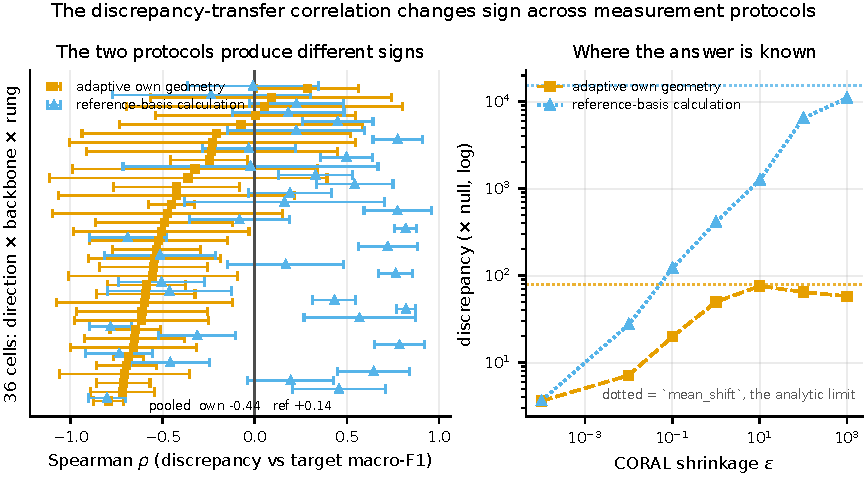
\includegraphics[width=\textwidth]{frame_dependence.pdf}
  \caption{Left: Spearman $\rho$ between a layer's marginal discrepancy and its
    target macro-F1 under two stated measurement protocols, for all 36
    (direction $\times$ backbone $\times$ rung) cells. Right: the analytically
    known CORAL map limit. The contrasting trajectories show measurement
    sensitivity; they do not identify one protocol as correct.}
  \label{fig:frames}
\end{figure*}

The mean of the cell-and-seed correlations is $-0.444$ in each rung's adaptive
own geometry and $+0.142$ in the reference-basis calculation. These opposite
signs describe the fixed sweep. Correlations share seeds and feature sets, so an
interval treating all cell-and-seed values as independent is not an inferential
justification for the sign change. Descriptively, 11 of the 36 individual cells
have uncorrected intervals on opposite sides of zero; this count is not used as
an independent significance claim.

The two statistics use the same features, layers and target scores. They differ
in their basis and bandwidth rule. \textbf{The correlation is therefore not
invariant to the stated measurement protocol.} The runs do not identify a
universally correct protocol. They show why a discrepancy--transfer correlation
must state its coordinate basis and bandwidth rule before it can be compared
with another report.

There is a second gap, and it runs the same way. The generalisation bound that
licenses treating discrepancy reduction as progress is stated over a
\emph{classifier-induced} divergence, defined on the symmetric difference of the
hypothesis class (Section~\ref{sec:related-alignment}). A kernel MMD at a fixed
bandwidth is not that quantity: it is a property of the two feature samples
alone and knows nothing about the hypothesis class the learner will search.
Reducing it is therefore not, in itself, reducing the term the theory bounds.

\paragraph{A map limit with known form.} One case fixes the interpretation
independently of any discrepancy measurement. With each covariance regularised
as $C + \varepsilon\,\mathrm{tr}(C)/d \cdot I$, CORAL's map satisfies
\begin{equation}
  M \;\longrightarrow\; \sqrt{\mathrm{tr}(C_t)/\mathrm{tr}(C_s)} \; I
  \label{eq:coral-limit}
\end{equation}
as $\varepsilon$ grows, so the transform collapses to a global scalar rescale
plus a mean shift: \texttt{mean\_shift} with one extra degree of freedom. A
shrinkage probe confirms the approach on real features, with the relative
distance to the nearest scaled identity falling from $0.9254$ to $0.0049$ and
the fitted scalar converging on the predicted limit; supplementary
Section~S5 reports the trajectory. The limiting map is a source-only
transformation, so the shared-scale invariance in
Equation~\ref{eq:median-scale-invariance} does not apply to it. Knowing the
map's form does not fix the measured discrepancy, which is the point.

\paragraph{Recommendation.} We state the consequence as a recommendation rather
than as a characterisation of what other work does or does not report, which we
are not in a position to survey. \textbf{A reported reduction in discrepancy
should state the geometry in which the discrepancy was measured: the kernel
bandwidth and the basis, and how each was fixed.} Where the bandwidth is set by
a data-dependent rule such as the median heuristic, this matters because the
statistic adapts to a global rescaling of both samples
(Equation~\ref{eq:median-scale-invariance}). A source-defined fixed kernel is
one explicit comparison protocol, not a universal remedy; its saturation under
z-score is reported in supplementary Section~S4. An adaptive calculation
answers a different question and should be labelled with its basis and
bandwidth rule.

\subsection{Where source validation is informative}
\label{sec:results-aggregation}

Source-side validation is not uninformative in general, and the same frozen grid
shows it. Comparisons A1 and A2 in Table~\ref{tab:primary} both survive
correction. Replacing final-layer pooling with a fixed mid-stack layer is worth
$+0.0640$ $[+0.0541, +0.0748]$ forward and $+0.1439$ $[+0.1140, +0.1746]$
reverse; replacing it with a learned softmax over all 13 states is worth
$+0.0597$ $[+0.0504, +0.0702]$ and $+0.1096$ $[+0.0888, +0.1326]$. These effects
are larger than any difference \emph{among} the aligned rungs ($\le 0.0437$) and
smaller than the decision to align at all.

Usefulness on one search axis does not imply usefulness on another, and the
contrast is the point: the same criterion that separates layer settings cannot
separate the two translation arms at all. The failure is specific to a decision,
not a property of source validation as such.

\subsection{Robustness of the aligned-versus-unaligned contrast}
\label{sec:results-robustness}

The comparison that the selection result rests on is aligned versus unaligned,
so we report whether it depends on the label harmonisation the two corpora
require. RAVDESS distinguishes \texttt{calm} from \texttt{neutral} and CREMA-D
does not; the main analysis merges them. Two pre-specified controls, one
dropping RAVDESS \texttt{calm} and one additionally excluding \texttt{neutral}
to give a five-class task, both keep every aligned-versus-\texttt{none} contrast
positive, with positive paired 95\% intervals and positive global one-sided
lower bounds under a shared 12-contrast Bonferroni family. Forward improvements
range from $+0.0914$ to $+0.1059$ under the first control and $+0.0612$ to
$+0.0946$ under the second; reverse improvements range from $+0.1121$ to
$+0.1388$ and $+0.1310$ to $+0.1697$. \textbf{The aligned-versus-unaligned
conclusion is therefore not an artefact of the calm-to-neutral mapping.}
Supplementary Section~S1 gives both controls in full.

Three further analyses are reported in the supplement because they qualify the
scope of these results without supporting the central argument. Standard
label-shift correction reduces macro-F1 in 238 of 240 (record, estimator) pairs
despite a small prior divergence, which bounds what a prior-only correction can
do here but does not establish those corrections' assumptions for these corpora
(Section~S2). Class-conditional discrepancy remains nonzero after alignment
under both label mappings; it is a descriptive diagnostic, is not an estimate of
$P(y \mid x)$, and is not offered as an explanation of the similarity among
aligned rungs (Section~S4). A historical blending probe, in which the best
setting of the interpolation parameter is the one that turns blending off,
produced no result that affects the criterion audit (Section~S7). Per-class F1
and the corresponding confusion structure of the source-validated
configuration, which describe how that configuration distributes its errors
rather than what the criterion can identify, are reported in Section~S6.

\section{Discussion}
\label{sec:discussion}

\subsection{What the results imply for practice}
\label{sec:discussion-practice}

The diagnostics in Section~\ref{sec:decomposition} place the ladder results in
context, but do not identify a causal mechanism.

\paragraph{Why standardisation captures the observed gain.} The ladder and its one-sided bounds
show that per-dimension standardisation captures the observed improvement: no
more complex rung is shown to improve target macro-F1 in either direction.
The evaluated CORAL and affine MK-MMD maps do not yield a further gain. The
diagnostics report raw marginal and class-conditional MMD$^2$ in one
source-defined reference geometry. Their class-specific null effect sizes aid
finite-sample interpretation but are not divided by the marginal effect size.
The fixed-bandwidth z-score control saturates the RBF kernel, so it is reported
as a measurement limitation rather than a closeness result.

\paragraph{Why lower marginal discrepancy does not help further here.}
The MMD rungs can reduce their fitted marginal objective without improving the
task metric. The class-conditional diagnostic provides a descriptive account of
that mismatch, but it is not a direct estimate of $P(y \mid x)$.

This analysis is limited to these rungs and this corpus pair. Covariate-shift
correction is justified by the assumption that $P(y \mid x)$ is stable across
domains. Our diagnostics do not directly test that assumption. Observed
label-prior differences are small: the prior KL is $0.02235$ and $0.02541$
nats, and the standard corrections examined here \emph{hurt} in 238 of 240
cases, by $0.013$ to $0.24$ macro-F1, while the same estimators recover a
planted shift. This does not establish the absence of label shift, because these
corrections rely on class-conditional assumptions that the diagnostic does not
verify.

\paragraph{What a correct selection protocol would have to measure.} The
forward selection result establishes a specific failure: source-side validation
does not reliably separate unaligned from standardised features in that
direction. It does not establish the cause. The class-conditional diagnostic
motivates a target-side signal sensitive to variation beyond the marginal
objective, but it is not itself such a signal and it requires target labels.
We do not have an unsupervised alternative to offer. What any candidate signal
must do is separate configurations that source-side validation cannot, and
Section~\ref{sec:results-selection} shows how wide that gap is.

\subsection{Selection is where this actually bites}
\label{sec:discussion-selection}

Table~\ref{tab:headline} gives the practitioner-facing validated scores and the
oracle gaps. \textbf{The forward oracle gap is larger than the observed
alignment gain.} It describes the room between source-side selection and the
target-set maximum; it does not isolate a causal effect of source-side
selection.

The forward selection surface is specific rather than universal: source-side
validation is nearly blind to the alignment distinction in that direction and
selects an unaligned, below-chance configuration once. A practitioner following
the protocol uses no target labels and has no source-side indication of that
failure. By contrast, source-side validation is informative on the layer-depth
axis in a separate analysis; the present result is limited to the alignment
decision.

This is also the argument for reporting baselines beside every performance
number. Without the chance baseline, a below-baseline result reads only as a
weak score.

\subsection{Testing the conditional-shift explanation directly}
\label{sec:discussion-testing}

Our class-conditional diagnostic is not a direct test of conditional shift. It
compares $P(x \mid y)$ across corpora, whereas the covariate-shift assumption
concerns $P(y \mid x)$. The falsifiable prediction we could test; that
label-shift correction should not help under near-zero prior KL; passed,
and passed sharply. That rules out neither a conditional-shift mechanism nor
other explanations for the plateau, so we state what a direct test would take.

It would need paired data: the same speakers, or the same sentences, recorded
under both corpora's conditions, so that $P(y \mid x)$ can be estimated
separately in each domain without the corpus difference and the speaker
difference being confounded. Failing that, per-utterance perceptual ratings from
multiple annotators would let the conditional be compared where the label is a
distribution rather than a point. Neither exists for this pair, so the
diagnostic here motivates a direct test rather than supplying one.

\subsection{Limitations}
\label{sec:limitations}

\textbf{Two corpora, one language, two directions.} Every result is a statement
about RAVDESS and CREMA-D in English. We have not shown that the observed
pattern, marginal discrepancy declining without a further transfer gain,
appears elsewhere. A corpus pair with a genuinely large prior difference
would test the label-shift correction result much harder than this one does.

\textbf{Both corpora are acted.} Neither contains spontaneous speech. Acted
emotion is more prototypical and more clearly separated than spontaneous
emotion, so the absolute scores here are likely optimistic relative to
spontaneous data. Whether the observed pattern transfers is genuinely open:
acted and spontaneous corpora may differ in ways not represented by this pair.

\textbf{Modest absolute performance.} Validated macro-F1 of $0.3156$ and
$0.4994$ clears chance comfortably but falls well short of in-domain SER. We
report a controlled analysis, not a system, and nothing here should be read as a
recommended pipeline.

\textbf{The reverse direction is less precisely measured.} RAVDESS as target
supplies $624$ test utterances against CREMA-D's $3677$ to $3690$, so reverse
intervals are wider throughout; for the among-rung bound, about $1.8$ times.
Both directions are matched in source-training size only. Their
source-validation and target-adaptation sizes still differ, so source-training
size cannot explain the directional asymmetry but other data-quantity effects
remain possible; the asymmetry in \emph{precision} is directly explained by the
different target-test sizes.

\textbf{The Transformer arm is reduced-seed.} Two seeds, the primary direction
only, one inner-grid setting per rung. It is never pooled with the five-seed
families and its intervals are correspondingly wider.

\textbf{The MK-MMD rungs frequently fall back.} Optimisation reverts to its
warm start in $64.9\%$ of \texttt{mkmmd\_diag} runs and $55.2\%$ of
\texttt{mkmmd\_full} runs, so in the majority of cells the fitted map \emph{is}
the CORAL or diagonal warm start. This qualifies the negative result about the
evaluated affine MK-MMD maps: this optimiser, at this budget, does not beat
standardisation. A better-optimised MK-MMD map might do better; these runs do
not decide that question.

\section{Reproducibility}
\label{sec:reproducibility}

\subsection{Provenance machinery}
\label{sec:repro-provenance}

Every result row carries a \texttt{run\_id} that is a deterministic hash over
the 19 coordinates defining the run, so a row can be recomputed from its own
recorded contents without reference to the script that produced it. The
configuration is frozen against a git tag and the runner refuses to start when
the working configuration has drifted from it; results here carry
\texttt{grid-freeze-v3}. The result schema is versioned, and the analysis
refuses to read rows written under an older version rather than silently
coercing them.

The conditional-shift diagnostic reads target labels, which every other part of
the pipeline is forbidden to do. It is therefore isolated: it lives in a
separate module, its outputs are never written to the run schema, and an
executable assertion reads the source of the alignment, classifier, grid-runner
and blending modules to check that none of them imports it. The separation is
checked by running it, not by convention.

\subsection{Checks that came free}
\label{sec:repro-checks}

Four consistency checks fell out of the design rather than being run as
exercises. A duplicate worker recomputed 23 WavLM sweep cells and produced
\textbf{bit-identical} target scores. The 151 sweep runs that share coordinates
with main-grid rows agree on all 57 non-volatile fields, \textbf{zero mismatches
across 8607 values}. Recomputing every \texttt{run\_id} from its own recorded
coordinates reproduces the stored identifier in \textbf{5424 of 5424 retained
result rows}.
And the Stage 1 sweep and Stage 2 grid, run weeks apart under different
enumerations, agree at rung \texttt{none} to $0.3700$ against $0.3698$.

Across the retained result ledger, \textbf{0 of 5424 rows failed}: 0 of the
4,986 frozen confirmatory runs, and 0 of the 438 retained Stage~0, Stage~1 and
baseline rows. In addition, 0 of 2340 sweep rows and 0 of 120 probe rows failed,
and \textbf{0 of 99{,}720 classifier trials failed to converge}.

\subsection{Provenance ledger}
\label{sec:repro-retractions}

The supplementary provenance ledger records the withdrawn, narrowed and
reversed claims that led to the frozen protocol. It includes the supporting
run filters and explains why none of those earlier statements is used in the
present article. The main text reports the resulting confirmatory evidence and
the null results below; the ledger remains available for audit without
interrupting the empirical argument.

\subsection{Null results}
\label{sec:repro-nulls}

Reported because they are results rather than omissions. The evaluated affine
\texttt{mkmmd\_full} map reaches the lowest discrepancy in \emph{both}
geometries and is never the best rung. Label-shift correction does not help,
hurting in 238 of 240 cases. Searching $\lambda$ for the MK-MMD rungs is not
worth the compute: \texttt{source\_val} varies by $0.0066$ (diagonal) and
$0.0196$ (full) across the entire grid. And the depth-divergence effect above
does not generalise, at a pooled gap of $+0.00$ layers.

\subsection{What is released}
\label{sec:repro-release}

The code, the frozen configurations, the result files and the generated tables
and figures are released together. Every figure and table in this paper is
produced from the result files by script; none is drawn or typed by hand, so
none can drift from the numbers it depicts. A single generated document lists
every number the paper cites with its interval, its floor and the run filter
that produced it, including the null results above and the supplementary
provenance ledger.

\section{Conclusion}
\label{sec:conclusion}

In this controlled RAVDESS and CREMA-D case study, feature-space alignment
improves target macro-F1 by $+0.12$ to $+0.20$ across the two directions,
against chance baselines near $0.166$. No evaluated rung beyond per-dimension
standardisation shows a further target-macro-F1 gain. The evaluated CORAL and
affine MK-MMD maps do not change that result.

The diagnostics show that lower marginal discrepancy does not imply better
transfer here. After alignment the marginal term is at $0.010\times$ its
unaligned value while the class-conditional diagnostic is still at $0.07\times$.
This is not an additive decomposition or a direct estimate of $P(y \mid x)$,
but it shows that the class-conditional diagnostic does not fall at the same
rate as the marginal objective. Observed label-prior differences are small in
this pair, and the standard corrections examined here do not improve transfer.
The elaborate rungs reduce their objectives, but that reduction does not deliver
a further target-macro-F1 gain.

Three conclusions follow for this protocol. As shrinkage grows, CORAL approaches
a scalar-rescaled mean shift. In the forward direction, source-side validation
can miss the need for alignment and once returns a score below the chance
baseline. The forward oracle gap exceeds the observed alignment gain, although
it also includes target-set maximisation. Finally, the relationship between
discrepancy and transfer reverses sign with the geometry used to measure it.
That relationship is not invariant until the measurement frame is stated.

The data support a limited recommendation. In this corpus pair, evaluate
per-dimension standardisation before adding more complex affine alignment maps.
Report the chance baseline beside every score and distinguish source-selected
scores from target-set oracle scores. A third corpus, especially one with a
different elicitation design, is required before extending this recommendation.

What we cannot offer is an unsupervised target-side signal sensitive to the
variation that separates successful from unsuccessful configurations. A signal
that directly tests $P(y \mid x)$ without target labels would be valuable, but
the present diagnostics do not identify one or establish that it is sufficient.

\section*{Data availability}

RAVDESS \citep{livingstone2018ryerson} and CREMA-D \citep{cao2014crema} are
third-party corpora and are not redistributed. The repository contains the
manifest construction, label mapping, speaker-disjoint split derivation,
generated results, and scripts for every manuscript table and figure.

\section*{Code availability}

The code is available in the
\href{https://github.com/prashant290605/Speech-Emotion-Recognition}{public project repository}.

\section*{Funding}

This research received no specific grant from public, commercial, or
not-for-profit funding agencies.

\section*{Declaration of competing interest}

The authors declare no competing financial interests or personal relationships.

\section*{Ethics statement}

This study uses existing public corpora of acted emotional speech. It collects
no new human-participant data. The reported cross-corpus scores are evidence
about evaluation methods and are not evidence for consequential affective
inference.

\printcredits

\section*{Declaration of generative AI and AI-assisted technologies in the
manuscript preparation process}

During preparation of this work, the authors used OpenAI ChatGPT and OpenAI
Codex to assist with manuscript drafting, readability review, code scaffolding,
and software maintenance. The authors specified the experiments, reviewed and
edited the code and manuscript, verified results against generated artifacts,
and take full responsibility for the content.


\bibliographystyle{cas-model2-names}
\bibliography{refs}

\end{document}
